\documentclass[14pt]{beamer}
\usepackage[backend=biber, style=ieee]{biblatex}
\addbibresource{library.bib}
\usepackage{amsmath}
\usepackage[per-mode=symbol, scientific-notation=true]{siunitx}
\usepackage[final]{microtype}
\usepackage{graphicx}
\graphicspath{{images/}, {r_figures/}}
\usepackage{default}
\mode<presentation>

\title{Distributed State Estimation on the TurtleBot Platform}
\author{Matthew Swartwout}
\date{August 26th, 2016}

\begin{document}
\begin{frame}
    \titlepage
\end{frame}

\begin{frame}
\frametitle{Outline}
\tableofcontents
\end{frame}

\section{Introduction}
\begin{frame}
\frametitle{What is localization and state estimation?}
\begin{itemize}
\item Robot localization answers the question "Where am I?"
\item Use sensors to obtain information about environment
\item Many methods to convert sensor information $\rightarrow$ state estimate 
\end{itemize}
\end{frame}

\section{Problem Statement}
\begin{frame}
\frametitle{Problem Statement}
Our distributed state estimation has five goals:
\begin{enumerate}
\item Integrate the robot's sensor information with information from other robots
\item Allow for dynamic resizing of the distributed network
\item Use unmodified Unscented Kalman Filter (UKF)
\item No requirement for static landmarks or cooperation with other robots
\item Use standard ROS practices and constructs
\end{enumerate}
\end{frame}

\section{Background}

\begin{frame}
%\frametitle{Background}
\frametitle{State Estimation}
\begin{itemize}
\item State estimation is a fundamental problem of robotics. Without knowing its position a robot loses a lot of its usefulness.
\item The Kalman Filter is one of the most studied and used Bayesian filters for state estimation~\cite{Localization2003, Mohsin2014}
\item We use the UKF, which has better accuracy for nonlinear systems than the Extended Kalman Filter and plain Kalman Filter
\end{itemize}
\end{frame}

\begin{frame}
%\frametitle{Background}
\frametitle{Distributed State Estimation}
Why make a distributed system?
\begin{itemize}
\item Networked mobile robots are becoming more ubiquitous
\item Can reduce the number of sensors required per robot
\item Theoretically more resilient to malfunctions and attacks
\end{itemize}
\end{frame}

\begin{frame}
%\frametitle{Background}
\frametitle{Examples of Distributed Systems}
\begin{itemize}
\item Cooperative Positioning
    \begin{itemize}
    \item Coordinate actions between robots
    \item Often use one robot as static landmark while another moves
    \end{itemize}
    \vspace{14pt}
\item Represent multiple robots as end effectors of a single robot
\end{itemize}
\end{frame}

\section{Hardware Platform}
\begin{frame}
%\frametitle{Hardware Platform}
\frametitle{TurtleBot}
\begin{itemize}

\item Developed by the Open Source Robotics Foundation, Inc. as a low cost, educational mobile robotics platform.
\vspace{14pt}
\item We combined the TurtleBot 2 and 2e specification with some modifications
\end{itemize}
\end{frame}

\begin{frame}
%\frametitle{Hardware Platform}
\frametitle{TurtleBot Specifications}
\begin{itemize}
\item Yujin Robot Kobuki mobile base
\item Avent ZedBoard
\item Microsoft Kinect Camera
\item Asus Wireless Router
\item USB Hub
\end{itemize}
\end{frame}

\begin{frame}
%\frametitle{Hardware Platform}
\frametitle{Kobuki Mobile Base}
The Kobuki mobile base is an open-source differential drive robot base developed for use with ROS.

\begin{itemize}
\item \SI{0.7}{\meter\per\second} max velocity
\item \SI{5}{\kilogram} max payload
\item Cliff sensor detects drops greater than \SI{5}{\cm}
\item Climbs thresholds less than \SI{12}{\mm}
\item \SI{3}{\hour} runtime
\end{itemize}
\end{frame}

\begin{frame}
%\frametitle{Hardware Platform}
\frametitle{ZedBoard}
The Avnet ZedBoard is a single board computer featuring a Xilinx Zynq-7000 All Programmable System on a Chip.
\begin{itemize}
\item Dual-core ARM Cortex-A9 processor
\item Xilinx FPGA
\item 512~MB DDR3 RAM
\item HDMI \& VGA output
\item USB 2.0 and JTAG connections
\end{itemize}

We run Linaro 14.10, an ARM specific fork of Ubuntu 14.04.
\end{frame}

\section{Distributed State Estimation}
\begin{frame}
\frametitle{Distributed State Estimation}
\framesubtitle{Theory}
Our system uses Lidar scans to calculate the pose of other robots in the environment and then shares the calculated pose with the other robot.
\begin{align}
&\text{UKF output} \rightarrow \text{position}_\text{robot1} \\
&\text{Lidar scan} + \text{position}_\text{robot1} \rightarrow \text{position}_\text{robot2} \\
&\text{position}_\text{robot2} \rightarrow \text{UKF input}
\end{align}
\end{frame}

\begin{frame}
%\frametitle{Distributed State Estimation}
\frametitle{System Assumptions and Constraints}

\begin{itemize}
\item An arbitrary number independent mobile robots operating in a planar environment
\item Wireless communication abilities between some robots in the environment
\item No known static map of environment
\item GPS and a compass for localization in the world frame is available
\item Motion planning and control of other robots is unknown and unpredictable
\end{itemize}
\end{frame}

\begin{frame}
%\frametitle{Distributed State Estimation}
\frametitle{Coordinate Frames}
\begin{itemize}
\item base\_link
    \begin{itemize}
    \item Rigidly connected to center of Kobuki mobile base
    \item Describes position of parts of robot relative to other parts 
    \end{itemize}
\item odom
    \begin{itemize}
    \item Fixed continuous world frame
    \item Origin is starting point of robot
    \item $odom \rightarrow base\_link$ represents position relative to starting point
    \item Drifts over time
    \end{itemize}
\end{itemize}
\end{frame}

\begin{frame}
%\frametitle{Distributed State Estimation}
\frametitle{Coordinate Frames cont.}
\begin{itemize}
\item map
    \begin{itemize}
    \item Fixed world frame
    \item Represents position in a common global frame
    \item Robot position in map frame is subject to discrete jumps
    \item Not subject to drift over time
    \end{itemize}
\end{itemize}
\end{frame}

\begin{frame}
%\frametitle{Distributed State Estimation}
\frametitle{UKFs}
For our UKFs we used the robot\_localization package~\cite{MooreStouch2014, Moore}, the defacto Kalman Filter solution for state estimation in ROS. We did make any modifications to the source code.
\pause
\begin{itemize}
\item Continuous Filter
    \begin{itemize}
    \item Publishes the $odom \rightarrow base\_link$ transformation
    \item Input is wheel encoder odometry
    \end{itemize}
\pause
\item Discrete Filter
    \begin{itemize}
    \item Publishes the $map \rightarrow odom$ transformation
    \item Inputs are wheel encoder odometry, GPS, and external poses
    \end{itemize}
\end{itemize}
\end{frame}

\begin{frame}
%\frametitle{Distributed State Estimation}
\frametitle{Nodes}
\begin{itemize}
\item Robot
    \begin{itemize}
    \item Receives Lidar and calculates external poses
    \item Sends movement commands
    \end{itemize}
\item Move\_Base
    \begin{itemize}
    \item The ROS navigation stack
    \item Contains global and local planners
    \item Receives movement goals from robot node and executes them
    \end{itemize}
\item Filters
    \begin{itemize}
    \item Continuous filter
    \item Discrete filter
    \end{itemize}
\end{itemize}
\end{frame}

\begin{frame}
\frametitle{Other Nodes}
\begin{itemize}
\item Noise injection
\item GPS publication
\item Sensor recording
\item Simulation timer
\end{itemize}
\end{frame}

\begin{frame}
\frametitle{Communications}
For sharing external poses we implemented an Action Server. Each robot has an action server that receives external poses, and then publishes them as an input to the UKF.
\vspace{14pt}

Each robot is able to scan the available servers and detected when a new server/robot is present. The robot then creates a client for the other server, and maintains a list of clients for all other robots in the environment.
\end{frame}

\section{Noise Model}
\begin{frame}
\frametitle{Noise Model}
Gazebo is an almost noise-free simulation, so we must add noise to create a realistic simulation.

\vspace{14pt}
We add noise to:
\begin{itemize}
\item Odometry
\item GPS
\item Lidar
\end{itemize}
\end{frame}

\begin{frame}
\begin{figure}
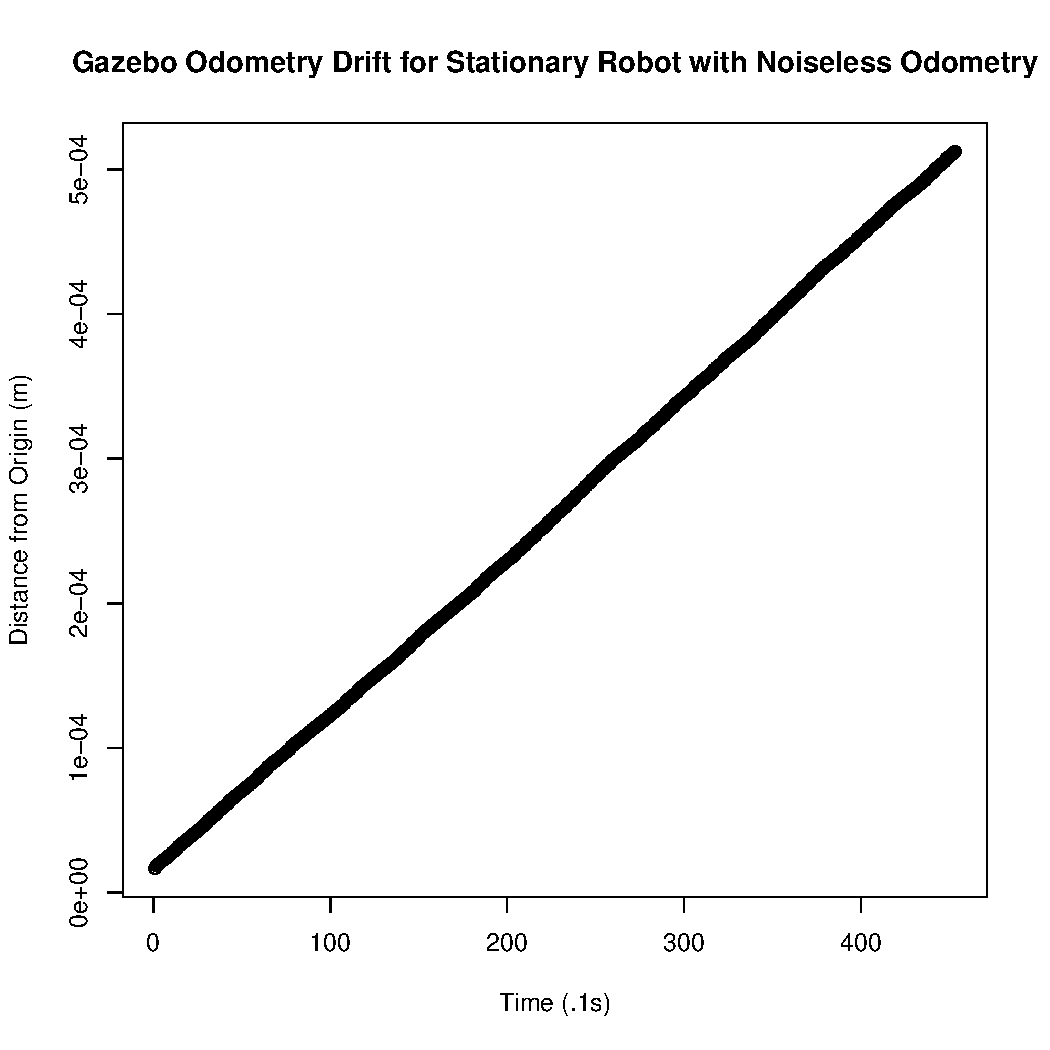
\includegraphics[keepaspectratio, scale=0.3]{gazebo_odom_drift}
\caption{Gazebo Odometry Drift for a Stationary Robot Over \SI{1}{\minute}. Drift is approximately \SI{3}{\cm\per\hour}.}
\label{fig:gazebo_odom_drfit}
\end{figure}
\end{frame}

\begin{frame}
\frametitle{Odometry Model}
For the odometry, the noise model was taken from Probabilistic Robotics by \textcite{ProbabilisticRobotics}. In Table 5.6 they show the algorithm for sampling from $p(x_t \mid u_t, x_{t-1})$, where $x_t$ represents the pose at time $t$ and $u_t$ represents the odometry measurement received.

\vspace{14pt}
This table is reproduced on the next slide.

\end{frame}

\begingroup
\footnotesize
\begin{frame}
\frametitle{Odometry Model Algorithm}
\begin{align}
&\delta_{\text{rot1}} = \text{atan2}(\bar{y}' - \bar{y}, \bar{x}' - \bar{x}) - \bar{\theta}\\ 
&\delta_{\text{trans}} = \sqrt{(\bar{x} - \bar{x}')^2 + (\bar{y} - \bar{y}')^2}\\
&\delta_{\text{rot2}} = \bar{\theta}' - \bar{\theta} - \delta_{\text{rot1}}\\
\notag \\
&\hat{\delta}_{\text{rot1}} = \delta_{\text{rot1}} - \textbf{sample}(\alpha_1\lvert\delta_{\text{rot1}}\rvert + \alpha_2\delta_{\text{trans}})\\
&\hat{\delta}_{\text{trans}} = \delta_{\text{trans}} - \textbf{sample}(\alpha_3\delta_{\text{trans}} + \alpha_4(\lvert\delta_{\text{rot1}}\rvert + \lvert\delta_{\text{rot2}}\rvert)\\
&\hat{\delta}_{\text{rot2}} = \delta_{\text{rot2}} - \textbf{sample}(\alpha_1\lvert\delta_{\text{rot2}}\rvert + \alpha_2\delta_{\text{trans}})\\
\notag \\
&x' = x + \hat{\delta}_{\text{trans}}\cos(\theta + \hat{\delta}_{\text{rot1}})\\
&y' = y + \hat{\delta}_{\text{trans}}\sin(\theta + \hat{\delta}_{\text{rot1}})\\
&\theta' = \theta + \hat{\delta}_{\text{rot1}} + \hat{\delta}_{\text{rot2}}\\
\notag \\
&return \ x_t = (x', y', \theta')^T
\end{align}
\end{frame}
\endgroup

\begin{frame}
\frametitle{GPS Noise Model}
\begin{itemize}
\item For GPS noise, we consulted an FAA study about the accuracy of GPS receivers~\cite{FAAGPS}.
\item This study showed that the GPS error fit a 95\% confidence interval of \SI{3.351}{\meter}.
\item Assuming this data is normally distributed, this gives a standard deviation of \SI{1.71}{\meter}.
\item We further assumed a mean of 0 for the error
\end{itemize}


\end{frame}
\begin{frame}
\frametitle{GPS Algorithm}
The algorithm for taking an odometry reading from Gazebo, $\bar{x}$, and the robot's initial position and creating a noisy GPS signal in the map frame.
\begin{align}
&x = x_{initial} + \bar{x}\\
&y = y_{initial} + \bar{y}\\
\notag \\
&horiz_{error} = \textbf{sample}(1.71)\\
&\theta = \textbf{$sample_{uniform}$}(0, 2\pi)\\
\notag \\
&x' = x + horiz_{error}\cos(\theta)\\
&y' = y + horiz_{error}\sin(\theta)
\end{align}
\end{frame}

\begin{frame}
\frametitle{Lidar Noise}
Our Lidar is simulated using a Kinect camera. To create noise in the Lidar we add noise to the Kinect camera in Gazebo.

\vspace{14pt}
Per the Gazebo Sensor Noise Tutorial~\cite{GazeboSensorNoise} recommendation, we used a mean of 0 and standard deviation of 0.007 for our camera's noise parameters.
\end{frame}

\begin{frame}
\frametitle{Pose Estimate Error}
The calculated poses of other robots have two sources of error.
\begin{itemize}
\item The external pose is calculated in reference to the robot's own noisy pose
\item The Lidar does not hit the direct center of the robot. This has a maximum error of \SI{0.2}{\meter}, and testing shows a mean error of \SIrange{0.05}{0.1}{\meter}
\end{itemize}
\end{frame}

\section{Results}
\begin{frame}
\frametitle{Control Group Results}
Control group testing of the continuous filter in a noiseless environment shows the localization systems functions correctly.

\begin{itemize}
\item Stationary Robot
    \begin{itemize}
    \item Max position error = \SI{.000002}{\meter}
    \item Max yaw error = \SI{.0001}{\radian}
    \end{itemize}
\item Mobile
    \begin{itemize}
    \item Max position error = \SI{.0001}{\meter}
    \item Mean yaw error = \SI{.001}{\radian}
    \end{itemize}
\end{itemize}
\end{frame}

\begin{frame}
\frametitle{Noisy Individual Results}
Next, we tested a single robot in a noisy environment. We saw expected drift with the mobile robot for the continuous filter, and no drift but a noisy estimate for the distributed filter. The stationary robot remained relatively noise free.
\end{frame}

\begin{frame}
\frametitle{Noisy Individual Results, cont.}
\begin{itemize}
\item Stationary Robot
    \begin{itemize}
    \item Continuous Filter
        \begin{itemize}
        \item Max position error = \SI{.00001}{\meter}
        \item Mean yaw error = \SI{.0001}{\radian}
        \end{itemize}
    \item Discrete Filter
        \begin{itemize}
        \item Max position error = \SI{.00001}{\meter}
        \end{itemize}
    \end{itemize}
\item Mobile Robot
    \begin{itemize}
    \item Continuous Filter
        \begin{itemize}
        \item Max position error = \SI{28.697}{\meter}
        \item Mean yaw error = \SI{.029}{\radian}
        \end{itemize}
    \item Discrete Filter
        \begin{itemize}
        \item Mean position error = \SI{1.366}{\meter}
        \item Max position error = \SI{6.037}{\meter}
        \end{itemize}
    \end{itemize}
\end{itemize}
\end{frame}

\begin{frame}
\frametitle{Noisy Group Results}
Finally, we simulate two mobile robots operating together and sharing external pose calculations between themselves.

\vspace{14pt}
\begin{itemize}
\item Distributed Filter
    \begin{itemize}
    \item Mean position error = \SI{.954}{\meter}
    \item Max position error = \SI{4.213}{\meter}
    \end{itemize}
\end{itemize}

Group operation reduced mean and max position error by 30\%.
\end{frame}
\section{Conclusion}

\begin{frame}[allowframebreaks]
\frametitle{Conclusion}
We had five goals from our Problem Statement:

\vspace{14pt}
\begin{enumerate}
\item Integrate the robot's sensor information with information from other robots
\begin{itemize}
\item Created Action Server infrastructure to communicate pose information between robots
\item Used UKFs to allow easy integration of external information
\item Operating with one other robot reduced mean and max position error by 30\%
\end{itemize}
\framebreak
\vspace*{14pt}
\item Allow for dynamic resizing of the distributed network
    \begin{itemize}
    \item Action Server infrastructure allows for detection of servers and creation of clients on demand
    \end{itemize}
\vspace{14pt}
\item Use unmodified Unscented Kalman Filter (UKF)
    \begin{itemize}
    \item Used robot\_localization package
    \end{itemize}
\framebreak
\item No requirement for static landmarks or cooperation with other robots
    \begin{itemize}
    \item System does not assume control or predictability of other agents
    \item Seamless transition between using own odometry and external poses
    \item All measurements taken while moving and published on demand
    \end{itemize}
\framebreak
\item Use standard ROS practices and constructs
    \begin{itemize}
    \item TurtleBot platform is well-documented and provides packages for almost everything
    \item Uses standard ROS navigation stack
    \item Uses robot\_localization for UKF implementation
    \item Kobuki mobile base is built for ROS and has published control packages
    \item No custom communications systems
    \end{itemize}
\end{enumerate}
\end{frame}

\section{Future Work}
\begin{frame}
\frametitle{Future Work}
\begin{enumerate}
\item Physical testing - We implemented solo autonomous navigation on the TurtleBot, but need to test group operation
\item Multimaster - A multimaster system (multimaster\_fkie or rocon) implementation will make this truly distributed and not decentralized
\item Implement secure Kalman Filter algorithms
\end{enumerate}
\end{frame}

\section{References}
\begin{frame}[allowframebreaks]
\frametitle{References}
\printbibliography
\end{frame}
\end{document}
